\documentclass[a4paper, oneside]{thesis}

\usepackage[utf8]{inputenc}
\usepackage[T1]{fontenc}

%for including full pdf pages
\usepackage[]{pdfpages} 

%%%%%%%%%%%%%%%%%%%%%%%%%%%%%%%%%%%%%%%%%%%%%%%%%%%%%%%%%%%%%%%%%%%%%%%%%%%%%%%%%%%%%%%%%%%%%%%%%
% DOCUMENT METADATA

\title{A computer-based learning environment aimed for students at the 3rd and 4th grade level}
\thesistype{Bachelor's Thesis}

\author{Florian Bütler}
\email{flbuetle@ethz.ch}

\institute{Chair of Information Technology and Education \\[2pt]
ETH Zürich}

\supervisors{Prof.\ Juraj Hromkovič}

% Optionally, keywords and categories of the work can be shown (on the Abstract page)
%\keywords{Keywords go here.}
%\categories{ACM categories go here.}

\date{\today}

%%%%%%%%%%%%%%%%%%%%%%%%%%%%%%%%%%%%%%%%%%%%%%%%%%%%%%%%%%%%%%%%%%%%%%%%%%%%%%%%%%%%%%%%%%%%%%%%%

\begin{document}

\frontmatter % do not remove this line
\maketitle

\cleardoublepage

\begin{acknowledgements}
	prof hrom kovic

team of abz for feedback

proofreaders

\TODO{}
\end{acknowledgements}


\begin{abstract}
	a brief introduction describing the discipline that the paper belongs to
a clear and concise statement of your problem
a brief explanation of your solution and its key ideas
a brief description of the results obtained and their impacts
\end{abstract}

\tableofcontents

\mainmatter % do not remove this line

% Start writing here
\chapter{Introduction}

\section{Motivation and Background}

With the introduction of Lehrplan 21 Computer Science became an integral part of the Swiss education curriculum \cite{Lehrplan21}. Pupils learn to understand the basic concepts of Computer Science and how to use them for problem solving. These concepts include methods on how to process, evaluate and summarize data, how to securely communicate and how to develop solution strategies for simple problems of information processing \cite{MedienUndInformatik}. The Education and Counselling Center for Computer Science Education at ETH Zürich \cite{ABZ} supports schools to teach these concepts among others by providing teaching resources and learning environments.

\section{Goals}

The main goal in this bachelor thesis is to implement tasks and riddles based on the textbook “einfach Informatik 3/4”, that will be published in spring 2021 \cite{EinfachInformatik}, in a computer-based learning environment that teaches the following concepts:

\begin{itemize}
    \item representing information with symbols,
    \item keeping information secret and
    \item learning from data
\end{itemize}

for pupils in the second cycle i.e the third and fourth grade of elementary school.
Along with solving tasks and riddles about the mentioned topics the ability of reading, writing, counting and calculating is trained as well.

\section{Related Work}

\TODO{maybe: about other learning environments}

\section{Outline}

This report start with the architecture of the computer based learning environment and its core implementation. Next it dedicates a chapter to each of the aforementioned concepts. Each chapter explains first how the concept is thought by hands-on exercises, then it gives an in-depth technical insight on how these exercises are implemented. At this point it is needed to be mentioned that the shown code might be simplified to highlight the intersting aspects, improve readability and to keep this report consise. Testing and Continous integration of the project is discussed before, finally, the report ends with a conclusion of the project.

\chapter{Architecture}
\label{chapter:architecture}

\section{Introduction}
\label{section:introduction}
\TODO{mention GitLab repo}

\section{TypeScript}
\label{section:typescript}
JavaScript had its publication in 1996, is a scripting language and is intended to be used in browsers to extend the possibilities of HTML and CSS. It can dynamically manipulate HTML and CSS, validate user data, send and receive data without reloading the page and much more.
TypeScript extends JavaScript by adding types and can be used anywhere JavaScript runs, because TypeScript code is transformed to JavaScript code by the TypeScript compiler. It provides a way to describe what type a variable has and helps to catch errors before the code is run. Moreover, TypeScript adds among others the concepts of method signatures, type interference, interfaces, enummerations and tuples. \cite{Typescript}.

\section{Vue.js}
\label{section:vuejs}
Vue.js is not developed by a company, but by Evan You and was first published in 2014. It is an alternative to Angular and React and was supossed to be a lightweight version of Angular. Vue.js is also based on reusable components, each having its own HTML, Javascript and CSS.
At the point the development of this project started, Vue.js version 3 was already published. However, Vue.js version 2 is used in this project, because the ecosystem has no caught up yet and many libraries only work with version 2 at the moment \cite{Vue}.

\subsection{Components}
Components are named resuable Vue.js instances and have the advantages that the structure, functionality and style of an element is implemented once and can then easily be used multiple times. Therefore each component has a parent (except from the root component) and possibly multiple child components forming a tree structure \cite{Vue}. 

\subsection{Communication between Components}
Communication between a parent and a child component happens from the parent to the child by properties and from child to parent by events. Properties are custom attributes that pass data from the parent to the child component. Events are emitted by a child component, can carry data and a parent can listen and react upon receiving an event from a child component \cite{Vue}.

\subsection{Best Practices}
The following list represent the best practice that were followind in this project. To see examples for each best pratice visit the Vue.js style guide  \cite{VueStyleGuide}.

\begin{itemize}
    \item Properties should be as detailed as possible and at least have a type.
    \item Always use \code{key} with \code{v-for} to maintain the internal component state.
    \item Avoid \code{v-if} with \code{v-for}
    \item Only the top-level \code{App} component and layout components should have global styles. All other components should always have scoped styles i.e the styles is only used within the component.
    \item Each component is in its own file.
    \item Filenames are in Pascal-Case.
    \item Components without any content should be self-closing e.g \code{<Component />} instead of \code{<Component><Component/>}.
    \item Components name casing in templates is PascalCase.
    \item Properties name casing is camelCase.
    \item Elements with multiple attributes should span multiple lines, with one attribute on each line.
    \item Component templates should only contain simple expressions. Complex expressions should be moved into computed properties or methods.
    \item Element attribute values should be quoted.
    \item Directive shorthands are always used.
    \item Element attributes should be ordered consistently.
    \item Components should be ordered like \code{<templates>}, \code{<script>} and \code{<style>}.
    \item Element selectors should be avoided with \code{scoped}
    \item Properties and events should be used for parent-child communication.
\end{itemize}

\section{Structure}
\label{section:structure}
The code for the project is located in the \textbf{src} folder. The \textbf{src} folder has the following content: 

\begin{itemize}
    \item \textbf{assets} - all the images and videos used in components
    \item \textbf{components} - all components of the project that are not a view
    \item \textbf{router} - everything in Vue.js is a component, but not everything is page. A page needs a route e.g. \code{/settings} and this folder contains all routes of the project. Components with a route are called \textbf{routed}
    \item \textbf{views} - all routed components
\end{itemize}
\TODO{structure in components}

The \textbf{tests} contains unit, snapshot and End-to-End tests for the project \ref{chapter:testingAndCI}. The \textbf{tests} contains the following:

\begin{itemize}
    \item \textbf{unit} - all unit and snapshot tests
    \item \textbf{e2e} - all e2e tests
\end{itemize}

\TODO{move following into own chapter and add implementation details}
\section{Basic functionality}
\label{section:basicFunctionality}

\subsection{Home Screen}
The home screen is a view and is the first page seens when visiting the learning environment. It has a simple structure: For each available exercise there is a card with an image to illustrate the exercise and its title. The basic ideas for the images are taken from the text book, but most of the time needed some simple photoshopping to make it represent the task reasonably.

\subsection{Game Mixin and Game Interface}

\subsection*{Game Mixin}
Mixins can be used to reuse functionality over different Vue components. When a component uses a mixin, all functionalities of the mixins are mixed into the component. All exercises use the \code{GameMixin} containing mostly the functionality on start and evaluate an exercises. Additionally, a function to generate a random number exists to mock random number generation in tests. More on that later.

\subsection*{Game Interface}
Each exercises implements the GameInterface. This ensures that exercise specific functionality like starting and evaluating the exercise is implemented and can be used in the \code{GameMixin}.

\begin{lstlisting}[language=TypeScript,caption={GameInterface},label={lst:gameInterface}]
interface GameInterface {
    isInitialized(): boolean;
    start(): void;
    isCorrect(): boolean;
}
\end{lstlisting}

\subsection{General Purpose Components}
The following presented components are components that are heavily reused. Most of them are part of the user interaction system since all exercises need some kind of user interaction elements.
\TODO{images for each component}
\TODO{maybe elaborate on technical details like passing events}

\subsection*{Game}
The Game component is an essential
\TODO{image about component tree structure}

\subsection{Event Bus}
Sometimes components are not in a direct parent-child relationship and still need to communicate. This can still be achieved by passing properties and emitting events, but evolves quickly into an unclear structure. To tackle this problem one can use an event bus. 
The event bus is a vue instance that allows to to emit an event in one component and listen for that event on another component. To use the event bus, a component simply needs to import the instance and can emit or listen for event on the usual way. This functionality is necessary between the game buttons and each exercise.

\subsection*{Game Buttons}
Every exercise needs a \textbf{check exercise} and a \textbf{next exercise} button to first check a given solution to an exercise and let the system check it and second to get to the next exercise.

\subsection*{Undo Button}
The Undo button simply restores the current exercise initial conditions, so one can retry it again.

\subsection*{Trashcan}
The Trashcan is an area where elements can be dropped to remove them. For example when pupils are asked to remove a letter from a word, they can either move the letter to this area and drop it or first click the element and then the trashcan are to remove it.

\subsection*{Difficulty Levels}
Some exercises have multiple difficulty levels. For those exercise the Difficulty component is used to change the level. This component gives the possibility to choose to up to three different difficulty levels indicated by an increasing amount of beavers on the button and a title.

\subsection*{Tutorial}
To introduce an exercise to the pupils the title of the exercise and a short instruction is not enough. Therefore for each exercise there is a detailed explanation of the background and purpose and a tutorial video. The tutorial video show an example run of first give a wrong solution, restart the exercise and finally give the correct solution.
The tutorial video were recorded by a screen capture tool and the moves on how to solve the exercise are done programmatically. The reason for this is that moving the mouse by hand to solve the exercise introduces a jitter to the mouse movement. The tutorial on the other hand should show clearly and without any hesitation the way on how to solve the exercise. Since this cannot be done by an average human being, the mouse movement is done programmatically. Each graphical element part of the exercise has an ID and one can give a list of IDs that should be visited in a run. For some this is straight forward.
\REMARK{possible to elaborate more on how to generate the ID list}

\section{Styles}
\label{section:styles}
\TODO{}
\chapter{Concept - Representing Information with Symbols}
\label{chapter:representingInformationWithWymbols}

\section{Similar Words}
\label{section:similarWords}

Representing information with symbols is a fundamental concept of Computer Science as information should be displayed clearly and concisely. Words can be seen as a sequence of symbols, namely a sequence of letters. The examples given in this section are in German, since the final application is in German as well.

In order to transmit information, it needs to be encoded in a word and sent to the destination.  The receiver needs to be able to decode and make sense of the transmitted information, even tough the word might contain errors such as spelling mistakes. To achieve this, sender and receiver agree on a list of used words. Each pair of words from this list has a minimal editing distance. 

The editing distance is the amount of operations that need to be done to transform a word in another by applying a sequence of operations. The operations are deleting, inserting and changing a letter \cite{AnD}.

\begin{example}
    The editing distance between \code{BACH} and \code{FACH} is 1, since changing the first letter from \code{B} to \code{F} transforms the first word into the second.
\end{example}

If sender and receiver agree on a list of words with a minimal pairwise editing distance and to only transmit words from this list, then the receiver can still uniquely determine what word the sender has sent, even when an error has been made. The receiver calculates the minimal editing distance between the received word and each word of the list and chooses the word with the smallest editing distance. The receiver assumes that this was the word the sender originally sent.

\subsection{Exercises}

The purpose of the \nameref{section:similarWords} exercises is to learn particular operations. An exercise is dedicated to one of the following operations: adding, changing and removing a letter from a word. Additionally, an exercise about swapping adjacent letters in a word is included.

\subsection*{Adding a letter}
\label{subsection:addingLetter}

In the \nameref{subsection:addingLetter} exercise, pupils are presented a word and the alphabet from A to Z. Pupils are supposed to choose a letter from the alphabet and add it to the word to form a new valid word.

\begin{example}
    The word \code{ARM} is given. By adding the letter \code{D} before the first letter, the valid word \code{DARM} is formed.
\end{example}

\subsection*{Changing a letter}
\label{subsection:changingLetter}

In this exercise, pupils are again shown a word and the alphabet from A to Z. The pupils should select a letter from the alphabet, but this time, instead of adding it, the selected letter should replace a letter from the word itself to create a new valid word.

\begin{example}
    The word \code{BUCH} is given. By changing the first letter from \code{B} to \code{T} the new valid word \code{TUCH} is formed.
\end{example}

\subsection*{Removing a letter}
\label{subsection:removingLetters}

In the \nameref{subsection:removingLetters} exercise, pupils receive a word, from which they should remove a letter to form a new valid word.

\begin{example}
    The word \code{BAUCH} is given. By removing the third letter the new valid word \code{BACH} is formed.
\end{example}

\subsection*{Swapping adjacent letters}
\label{subsection:swappingLetters}

When typing on a keyboard, typing mistakes happen. This exercise is supposed to train the ability to spot a common mistake, where only two adjacent letters are swapped \cite{EinfachInformatik}.

The pupils are presented a word with swapped adjacent letters, which they need to identify and swap back to restore the original word. This exercise has two difficulty levels. On the easy level only one pair of adjacent letters is swapped and on the medium level two pairs of adjacent letters are swapped.

\begin{example}
    The word \code{BCAH} is given (easy level). By swapping the second and third letter the original word \code{BACK} is restored.
\end{example}

\subsection{Implementation}

\subsection*{Word List Generation}

The foundation of these exercises is to have a list of words and for each word a list of similar words. A similar word is a word into which the original word can be transformed by either adding, changing or removing letters within a given number of operations, i.e. editing distance. In this implementation the editing distance used is one. This means only one operation can be applied, either adding, changing or removing a letter. This makes generating a list of words the easy part. Basically any list of words will do the job, but they should be understandable for children. So the first step is to collect a list of child-friendly nouns. 

Not much more difficult, but much more expensive, is the computation of similar words. Given the list of child-friendly nouns and the list of allowed words, one can brute force a list of similar words by applying each transformation to every noun and checking whether the transformed word exists in the allowed word lists. The script to generate a list of similar words for each word and each operation is given in listing \ref{lst:similarWords}.

%TC:ignore
\begin{lstlisting}[language=Python,caption={Algorithm to generate a list of similar words in Python},label={lst:similarWords}]
for word in children_words:
  add = list()
  for pos in range(len(word) + 1):
    for letter in ALPHABET:
      w = word[:pos] + letter + word[pos:]
      if contains(allowed_words, w) and not w in add:
        add.append(w.upper())
  similar_words["add"][1][word.upper()] = add

  remove = list()
  for pos in range(len(word)):
      w = word[:pos] + word[pos + 1 :]
      if contains(allowed_words, w) and not w in remove:
          remove.append(w.upper())
  similar_words["remove"][1][word.upper()] = remove

  change = list()
  for pos in range(len(word)):
    for letter in ALPHABET:
      w = word[:pos] + letter + word[pos + 1 :]
      if contains(allowed_words, w) and not w in change:
        change.append(w.upper())
  similar_words["change"][1][word.upper()] = change
\end{lstlisting}
%TC:endignore

\begin{example}
  Examples of similar words for adding, changing and removing a letter from a word
  \begin{itemize}
    \item \nameref{subsection:addingLetter} - \code{ARM}: \code{ARME}, \code{ARMS}, \code{DARM}, \code{FARM}, \code{WARM}
    \item \nameref{subsection:changingLetter} - \code{BUCH}: \code{AUCH}, \code{BACH}, \code{BUSH}, \code{EUCH}, \code{HUCH}, \code{SUCH}, \code{TUCH}
    \item \nameref{subsection:removingLetters} - \code{BAUCH}: \code{AUCH}, \code{BACH}, \code{BUCH}
  \end{itemize}
\end{example}

Significantly more difficult is to generate a list of allowed words. Three different approaches were taken:

\begin{itemize}
  \item Using a list of approximately ten thousand nouns
  \item Collecting a list from online dictionary of allowed words of the well known word game Scrabble \cite{Scrabble}
  \item Generating a list from a spell checker
\end{itemize}

The first approach resulted in a word list with which exercises could be generated. However, the word list obviously didn't cover all possible words pupils could know. Therefore, the word list needed to be extended.

Hence the idea to create a list of words that are allowed in Scrabble came up. This seemed like a good idea until it showed that the online Scrabble dictionary does not include all valid words.
Collecting words from the Scrabble dictionary resulted in approximately thirty thousand words, each between two and 8 letters long.

Finally, the last approach was taken by generating a list of allowed words from a spell checker. A well-known and open-source spell checker is Hunspell. However, Hunspell doesn't have a list of all allowed words, but rather generates them from two files: the dictionary file and the affix file. The dictionary file contains a list of root words and applicable rules for each root word. The affix file stores a list explaining these rules. Each rule defines an operation that can be applied to a root word. The spell checker evaluates a word as correct if it can construct the word by applying rules to a root word \cite{Hunspell}.

Luckily, there exists a tool called \code{unmunch} in the Hunspell ecosystem that generates a list of words from the dictionary file and the affix file as easy as shown in listing \ref{lst:unmunch} \cite{HunspellGithub}.
In the end, a list of about one million allowed words was generated (without any word length limits). However, a drawback is that the word list does not contain any names from people, cities or any other instances. 

%TC:ignore
\begin{lstlisting}[language=Bash,caption={Bash command to unmunch a dictionary file and a affix file to a list of words},label={lst:unmunch}]
$ unmunch German_de_CH.dic German_de_CH.aff > wordlist.txt
\end{lstlisting}
%TC:endignore

The actual implementation of these exercise types is straight forward. Each exercise type displays a random word from the word list and each letter of the word is on a card to allow easy user interaction. Two exercise types, namely adding and changing a letter, need an alphabet. The \nameref{subsection:addingLetter} exercise is implemented in the \code{Add.vue} component (figure \ref{fig:addingLetter}) and shows arrows between each letter and at the beginning and end of the word, where pupils can add a new letter selected from the alphabet. The \nameref{subsection:changingLetter} exercise works similarly, but instead of having arrows, pupils can replace each letter themselves with a new letter selected from the alphabet (figure \ref{fig:changingLetter}). In the \nameref{subsection:removingLetters} exercise, pupils can move a letter to the trashcan to remove it (figure \ref{fig:removingLetter}). In the \nameref{subsection:swappingLetters} exercise, they can click on the arrows to change the order of the letters (figure \ref{fig:swappingLetters}).

\begin{figure} 
  \centering
  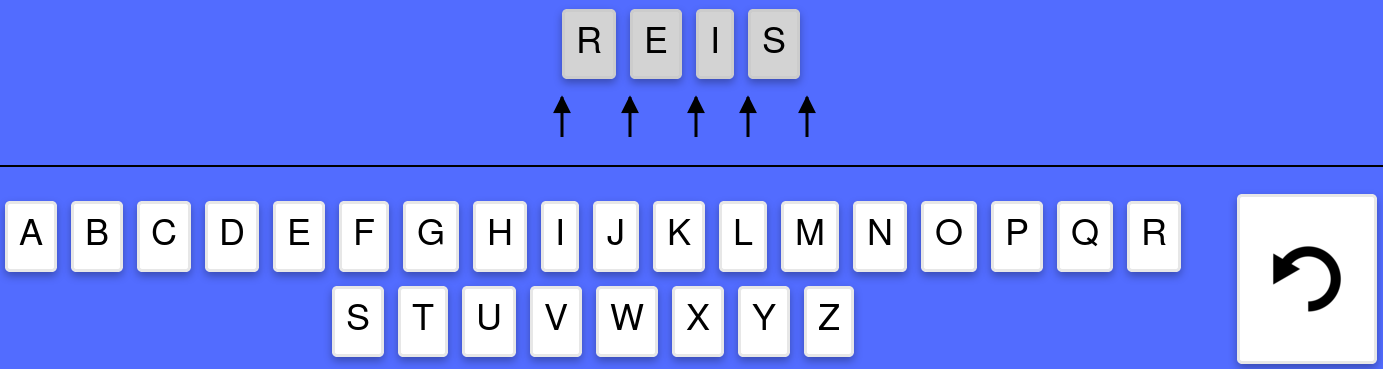
\includegraphics[width=1.0 \columnwidth]{figures/words_add.png}
  \caption{Adding a letter exercise} 
  \label{fig:addingLetter} 
\end{figure}

\begin{figure} 
  \centering
  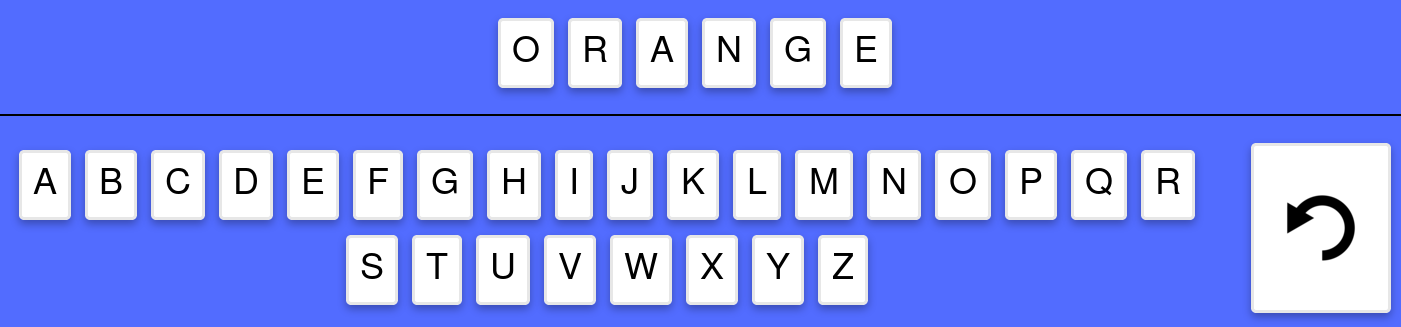
\includegraphics[width=1.0 \columnwidth]{figures/words_change.png}
  \caption{Changing a letter exercise} 
  \label{fig:changingLetter} 
\end{figure}

\begin{figure} 
  \centering
  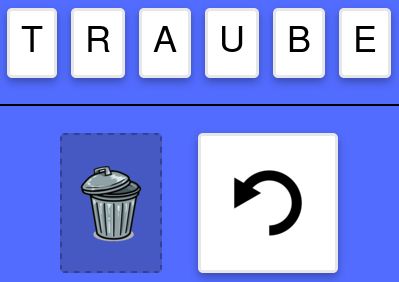
\includegraphics[width=0.3 \columnwidth]{figures/words_remove.png}
  \caption{Removing a letter exercise} 
  \label{fig:removingLetter} 
\end{figure}

\begin{figure} 
  \centering
  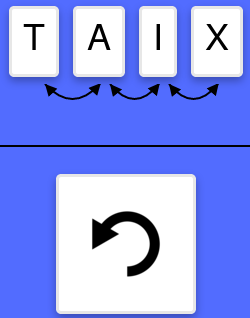
\includegraphics[width=0.2 \columnwidth]{figures/words_swap.png}
  \caption{Swapping letters exercise} 
  \label{fig:swappingLetters} 
\end{figure}

\section{Number Systems}
\label{section:numberSystems}

\subsection{Exercises}
\subsection*{Representing Numbers like the Maya}

Today, people are used to the decimal number system (base number 10), with 10 symbols. The Maya used a different number system with a base number of 20 i.e the vigesimal number system. It is believed that the Maya used their ten fingers and ten toes to count adding up to twenty. But instead of having a symbol for each number as in the decimal system, the Maya used three different symbols: zero (a turtle shell, belly side up), one (a dot) and five (a bar) \cite{Maya}. The Mayan representation of the decimal numbers from 0 to 19 can be found in figure \ref{fig:maya_numerals}.

\begin{figure} 
    \centering
    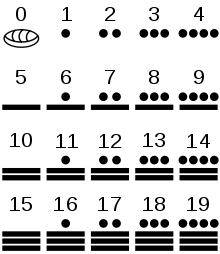
\includegraphics[width=0.3 \columnwidth]{figures/maya_number_system.png}
    \caption{Representation of the Maya numbers from 0 to 19} 
    \label{fig:maya_numerals} 
\end{figure}

The following exercises are supposed to familiarize pupils with a new number system, the Mayan number system. First, converting numbers between the decimal number system and the Mayan numbers is trained and then topped off with an exercise about adding two Mayan numbers.

\subsubsection*{Representing Mayan numbers}

A decimal number is presented to the pupils. They need to choose the correct amount of dots and bars representing the decimal number as shown in figure \ref{fig:maya_numerals}. For the purpose of simplicity, only decimal numbers between 1 and 19 are chosen.

\subsubsection*{Understanding Mayan numbers}

In this exercise the pupils learn to understand Mayan numbers. Again only decimal numbers between 1 and 19 are used. The pupils need to understand what Mayan number is shown and write down the decimal equivalent.

\subsubsection*{Adding Mayan numbers}

This exercise combines the previous two. The pupils need to understand the summands given in the Mayan number system, add them together and write down the sum in either the decimal number system or the Mayan number system. This exercise has two difficulty levels:

\begin{itemize}
  \item \textbf{easy} - the pupils have to calculate the sum as a number 
  \item \textbf{medium} - the pupils have to calculate the sum as a representation of numbers from the Mayan number system
\end{itemize}

\subsection*{Representing Numbers with Coins}

The following exercises introduce a new number system and train an already learned one: the binary number system and the decimal number system. Both number systems are practiced with coins and with numbers. The binary coins include the following numbers: 1, 2, 4, 8, 16, 32 and 64 (figure \ref{fig:binary_coins}). The decimal coins include 1, 2, 5, 10, 20 and 50 (figure \ref{fig:decimal_coins}). 

Overall, the same concepts are practiced for both number systems with the limitation that every binary coin can at most be used once.

\begin{figure} 
    \centering
    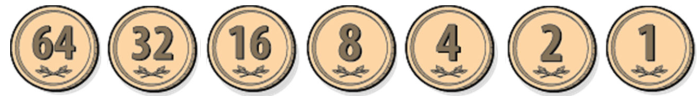
\includegraphics[width=0.5 \columnwidth]{figures/decimal_coins.png}
    \caption{Representation of the decimal coins} 
    \label{fig:decimal_coins} 
\end{figure}

\begin{figure} 
    \centering
    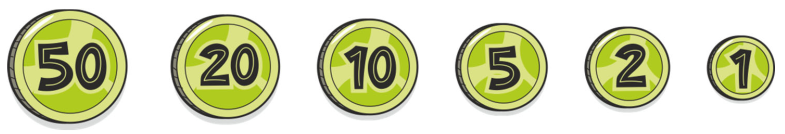
\includegraphics[width=0.5 \columnwidth]{figures/binary_coins.png}
    \caption{Representation of the binary coins} 
    \label{fig:binary_coins} 
\end{figure}

\subsubsection*{Conversion of a decimal number to its coin representation}

This exercise includes two difficulty levels:

\begin{itemize}
    \item Converting a decimal number to a coin representation, where the sum of all coins are equal to the decimal number
    \item Converting a decimal number to a coin representation, where the sum of all coins are equal to the decimal number \textbf{and} the amount of used coins is minimal.
\end{itemize}

\subsubsection*{Conversion of a number given in its coin representation to a decimal number}

A number given in its coin representation, either binary or decimal coins, has to be converted to a decimal number. 

\subsubsection*{Reducing the amount of used decimal coins while keeping the same sum}

Similar to the previous exercise, a sum in its coin representation is given and pupils have to display the same sum but with fewer coins. This exercise only makes sense for decimal coins since binary coins are always minimal.

\subsection{Implementation}

The conversion exercises from the decimal number system to either the Mayan, decimal coins or binary coins all share the same logic implemented in the \code{To.vue} component (figure \ref{fig:coinsTo}).
The same goes for the inverse direction (\code{From.vue} component, figure \ref{fig:coinsFrom}).

However, adding Maya numbers (\code{Addition.vue}, figure \ref{fig:mayanAddition}) and reducing the amount of used coins (\code{Swap.vue}, figure \ref{fig:coinsSwap}) require their own logic and are therefore implemented in their own components.

\begin{figure} 
  \centering
  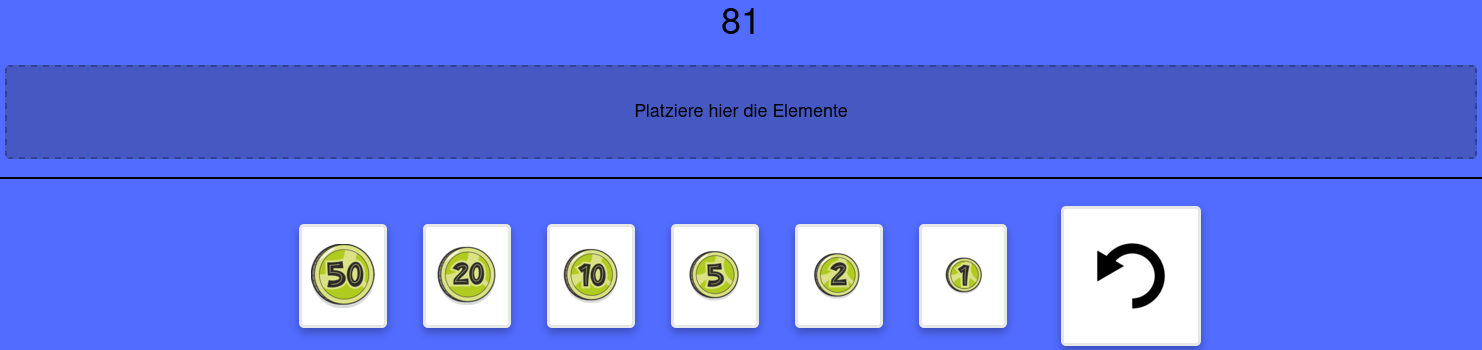
\includegraphics[width=1.0 \columnwidth]{figures/coins_to.png}
  \caption{Conversion of a decimal number to its coin representation exercise} 
  \label{fig:coinsTo} 
\end{figure}

\begin{figure} 
  \centering
  
\includegraphics[width=1.0 \columnwidth]{figures/coins_from.png}
  \caption{Conversion of a decimal number from its coin representation exercise} 
  \label{fig:coinsFrom} 
\end{figure}

\begin{figure} 
  \centering
  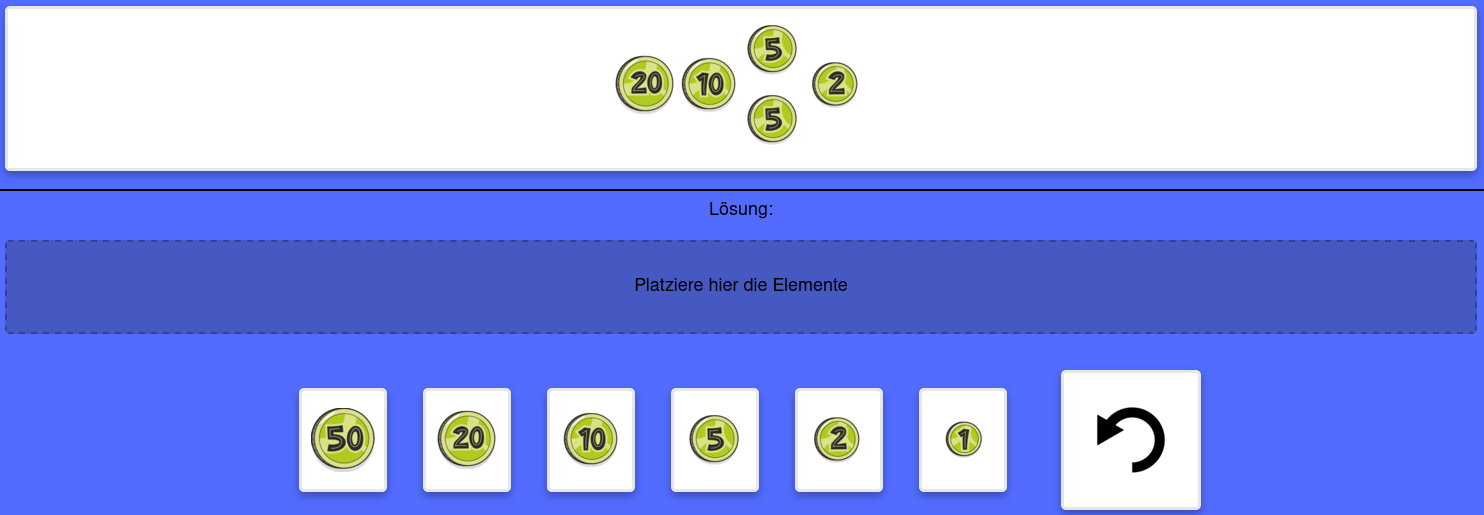
\includegraphics[width=1.0 \columnwidth]{figures/coins_swap.png}
  \caption{Reducing the amount of decimal coins in a given set of decimal coins exercise} 
  \label{fig:coinsSwap} 
\end{figure}

\begin{figure} 
  \centering
  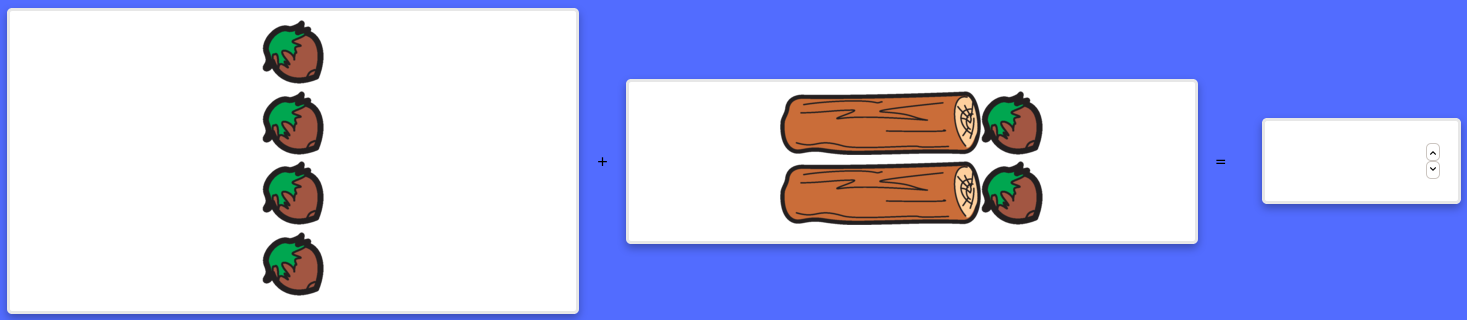
\includegraphics[width=1.0 \columnwidth]{figures/mayas_addition.png}
  \caption{Adding Mayan numbers exercise (easy)} 
  \label{fig:mayanAddition} 
\end{figure}

The \code{To.vue} component is simple. It shows a a random number between one and a number system specific limit:

\begin{itemize}
  \item \textbf{Mayan number system} - limit: 19
  \item \textbf{Decimal coins} - limit: 100
  \item \textbf{Binary coins} - limit: 100
\end{itemize}

The pupils need to select items (either nuts, sticks or coins) with the correct value and place them such that they sum up to the shown random number.

In addition, there is another difficulty level for the conversion to decimal coins, where the aim is to represent the displayed random number with as few decimal coins as possible. The algorithm to calculate the minimal amount of items necessary for a certain sum is given in listing \ref{lst:calcMinimalAmount} 


%TC:ignore
\begin{lstlisting}[language=TypeScript,caption={Calculate minimal amount of items needed to reach a certain number},label={lst:calcMinimalAmount}]
calcMinimalAmount(type: numbersystemType, number: number): number[] {
  const items = this.items(type);
  let i = 0;
  const minimalAmount = new Array<number>(items.length).fill(0);
  while (number > 0 && i < items.length) {
    const value = items[i].value;
    if (number >= value) {
      minimalAmount[i]++;
      number -= value;
    } else {
      i++;
    }
  }
  return minimalAmount;
}
\end{lstlisting}
%TC:endignore

The implementation for the \code{From.vue} component works in a similar fashion. This time a random number of items is generated. The pupils need to add up these items' values.

Both of these components at some point need to sum the items' values. It would be convenient to have a map where each item type maps to the amount of selected or shown items and a map where each item type maps to its value. However, due to Vue.js constraints, this is not possible, as the Map datatype is not reactive.

The Array datatype on the other hand is reactive. Therefore an array is used, where the first element represents the highest item value, and the last element represents the item with the lowest value. This introduces some tight coupling between the array storing the amount of items and the array storing the value of each item. The implementation to sum items is shown in listing \ref{lst:sumItems}.

%TC:ignore
\begin{lstlisting}[language=TypeScript,caption={Sum up items},label={lst:sumItems}]
sumItems(type: numbersystemType, items: number[]): number {
  if (items.length !== this.items(type).length) {
    throw Error(`array lengths do not match:  ${items} ${this.items(type)}`);
  }
  let sum = 0;
  for (let i = 0; i < this.items(type).length; i++) {
    sum += items[i] * this.items(type)[i].value;
  }
  return sum;
}
\end{lstlisting}
%TC:endignore

The \code{Swap.vue} component reuses some parts of the just mentioned components. It also generates a random amount of each item. The total amount of items is guaranteed to be reducible and pupils are asked to represent the same sum over all items but with fewer items. How such a configuration is achieved, is shown in listing \ref{lst:reducableItems}.

%TC:ignore
\begin{lstlisting}[language=TypeScript,caption={Generate a reducible item configuration},label={lst:reducableItems}]
do {
  this.generatedItems = this.generateItems(this.type);
} while (
  this.sumItems(this.type, this.generatedItems) >= this.limit(this.type) ||
  this.countItems(this.generatedItems) ===
    this.countItems(
      this.calcMinimalAmount(
        this.type,
        this.sumItems(this.type, this.generatedItems)
      )
    )
);
\end{lstlisting}
%TC:endignore

In the \code{Addition.vue} component all previously seen concepts come together. Two summands are generated, each with a random amount of items. The sum is guaranteed to not overshoot the limit of this number system. 
\chapter{Keeping Information Secret}

The previous chapter \ref{chapter:representing_information_with_symbols} was about representing information with symbols. This section is about keeping information secret.
Ciphers haven been used for thousands of years \cite{HistoryOfCryptography}. They are used to keep information secret from people, that are not supposed to have knowledge of it. Not encrypted information is called clear text. Once one encrypted a clear text, it is called a cipher text and only people who know how to decrypt the cipher text can read originally encrypted information.
The exercises in this section are introducing pupils to the concepts of ciphers.

\section{Cipher Texts from Reversed Letters}

\subsection{Concept}
The cipher used in these exercises is a simple mix up of letters and both directions are trained: encryption and decryption. In the decryption exercise, the pattern, on which the clear text was encrypted with, is shown. The pupils need to understand the pattern and move the letters in the cipher text accordingly to retrieve the clear text. The encryption exercise is set up analogously. Multiple difficulty levels are possible by changing the amount of moved letters.

\begin{example}
    The cipher text is \code{ULFSS} and the pattern is shown in figure \ref{fig:pattern}. By moving the letter in the cipher text according to the pattern, the clear text can be retrieved: \code{FLUSS}.
\end{example}

\begin{figure} 
    \centering
    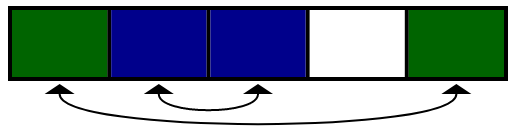
\includegraphics[width=0.4 \columnwidth]{figures/pattern.png}
    \caption{Pattern} 
    \label{fig:pattern} 
\end{figure}

\subsection{Implementation}

\section{Cipher Texts from New Characters}

\subsection{Concept}
Sometimes, only moving symbols in not enough to keep information secret. A better why is to substitute symbols with new symbols. These symbols may be letters, numbers or completly new symbols, that are solely invented for the purpose of encrypting information.
In the following exercises the last approach is followed. Again both direction, encryption and decryption, are trained. But this time, instead of having a pattern, there is a symbol table showing how the letters are encrypted. 

\begin{example}
    The cipher text is shown in figure \ref{fig:cipher_number} and the symbol table in figure \ref{fig:symbol_table}. By using the symbol table one can decrypt the cipher text to \code{52}.
\end{example}

\begin{figure} 
    \centering
    
\includegraphics[width=0.2 \columnwidth]{figures/cipher_number.png}
    \caption{Cipher text of an encrypted number} 
    \label{fig:cipher_number} 
\end{figure}

\begin{figure} 
    \centering
    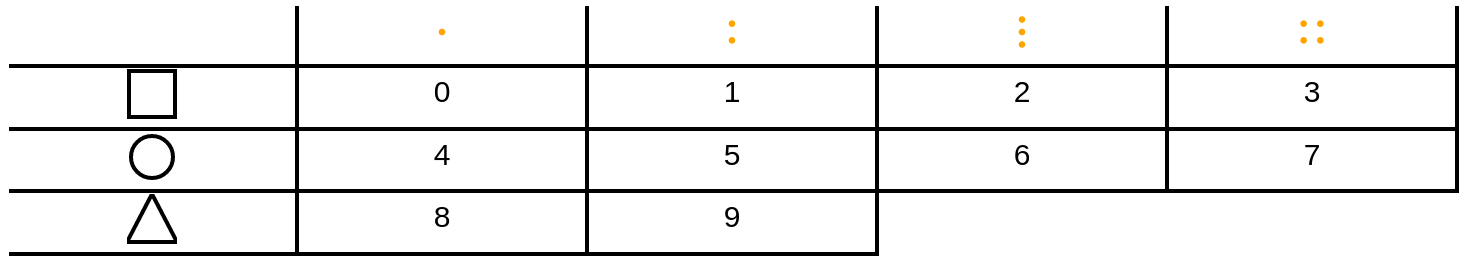
\includegraphics[width=1.0 \columnwidth]{figures/symbol_table.png}
    \caption{Symbol table to encrypt numbers} 
    \label{fig:symbol_table} 
\end{figure}

\subsection{Implementation}
% drawing on canvas
\chapter{Learning from Data}
\label{chapter:learningFromData}

The following exercises are logic-based, combinatorial puzzles. The idea is that pupils need to conclude the solution by a partially completed grid.

\section{Row of Trees}
\label{section:treeRow}

\subsection{Exercises}
The row of trees is a one dimensional grid i.e a row either of size 3 or 4. In every row there is exactly one tree of every height between 1 and 3 (Fig. \ref{fig:trees_3}) or 4 (Fig. \ref{fig:trees_4}) respectively. At both ends of the row the amount of tree visible from this end of the row is given.
Pupils are given an empty row with only the number of trees seen from both ends of the row and need to place a tree of each height such the aforementioned rules are met.

\begin{figure} 
    \centering
    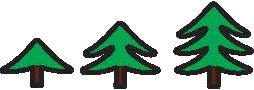
\includegraphics[width=0.4 \columnwidth]{figures/trees_3.png}
    \caption{Trees from height 1 to 3} 
    \label{fig:trees_3} 
\end{figure}

\begin{figure} 
    \centering
    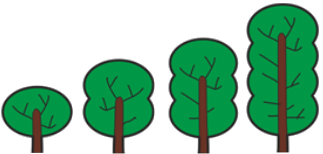
\includegraphics[width=0.4 \columnwidth]{figures/trees_4.png}
    \caption{Trees from height 1 to 4} 
    \label{fig:trees_4} 
\end{figure}

\begin{example}
    For a row of size 3, if given the value 2 for both ends of the row, then one possible solution to the puzzle is shown in figure \ref{fig:tree_row_example}.
\end{example}

\begin{figure} 
    \centering
    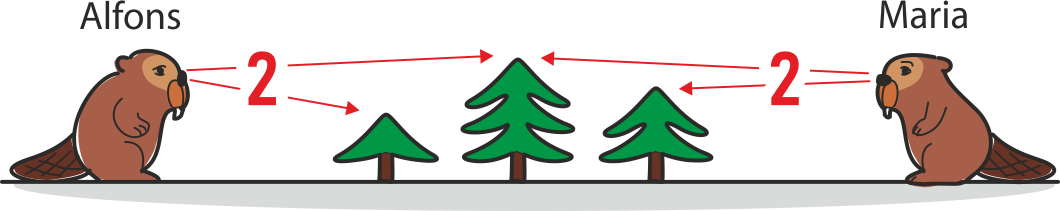
\includegraphics[width=0.8 \columnwidth]{figures/tree_row_example.png}
    \caption{Visualization of the puzzle solution from the tree row example} 
    \label{fig:tree_row_example} 
\end{figure}

\subsection{Implementation}

\section{Tree Sudoku}
\label{section:treeSudoku}

\subsection{Exercises}
Tree sudoku is similar to the well known traditional sudoko with the difference that trees of different heights are placed instead of numbers, and for end of every row and collumn the number of visible trees is given. Otherwise, the puzzle follows the same rules as the row of trees and is either of size 3x3 or 4x4.

\begin{example}
    An example of a 3x3 tree sudoku is shown in figure \ref{fig:tree_sudoku_example}
\end{example}

\begin{figure} 
    \centering
    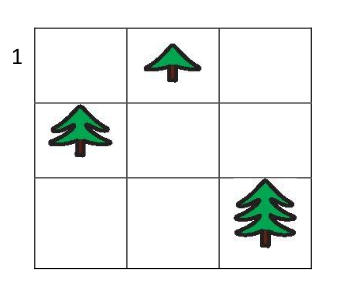
\includegraphics[width=0.4 \columnwidth]{figures/tree_sudoku_example.png}
    \caption{Example of an unsolved 3x3 tree sudoku} 
    \label{fig:tree_sudoku_example} 
\end{figure}
% https://www.bowdoin.edu/~sbarker/teaching/courses/ds/18fall/files/lab4.pdf

\subsection{Implementation}
% sudoku solver
\chapter{Testing and Continous Integration}
\label{chapter:testingAndCI}

Implemented funtionality should always be tested. Not only to ensure that is currently does what it is supposed to do, but also to avoid regression. Nothing is worse than introducing a bug by implementing a new feature with noticing it. Therefore in this project we use unit, snapshot and End-to-End test to avoid regression.
Moreover, all tests are always run upon each commit to the GitLab repository.

\section{Testing}
\label{section:testing}
For unit and snapshot testing Jest is used. Jest is a JavaScript testing framwork focusing on simplicity and is maintained by Facebook. It is supposed to require zero config and runs tests isolated and therefore can be paralellized \cite{Jest}. For End-to-End testing Nightwatch is used. Nighwatch is a Node.js powered End-to-End testing framework for web applications and websites. It supports testing in Chrome, Firefox and Edge, supports page object to easily abstract the content of a page and allows extending the framwork with custom commands \cite{Nightwatch}.

\subsection{Unit Testing}
\label{subsection:unitTesting}
Unit tests are usually used to verify the functionality of functions and work with the following concept: the tester has an input to a function and knows what the function should output for this input. The tester then compares the actual ouput of the function and compares it to the expected output. If those are not the same the test is evaluated as failed, and succeeded otherwise.
There are mainly two different categories of unit tests: black-box and white-box testing.

\subsection*{Back-box and White-box Testing}
Black-box testing is a testing method, where the tester does not know how a feature is implemented and has to think of cases by just using ones understanding of the feature. White-box testing on the other hand is a testing method, where the tester does know the implementation of the feature. Usually both kind of software testing is used. But since there are no software tester  (testers without any knowledge of the impelementation) involved in this project, only white-box testing is applied \cite{BlackBoxWhiteBoxTesting}.

\subsection*{Test Plan}

General purpose components are tested in its specialized functionality i.e wheter they react correctly on different user inputs. \TODO{maybe elaborate on that?}
The components representing an exercises are tested for:

\begin{itemize}
    \item Initial conditions hold
    \item Various exercise specific user inputs are handled correctly
    \item Restarting the exercise works as expected
    \item Starting next example restores the initial conditions
    \item Correct answer is accepted
    \item Incorrect answer is rejected
\end{itemize}

\subsection*{Code Coverage}
As mentioned before, unit test usually test a feature on the function level. To catch as many possible code paths and corner cases, the same function is tested multiple times with different inputs. 
A metric to judge the usefullness of a test suite is the code coverage. The code coverage shows how well a test suite covers the functionality. Usually, a coverage report includes:

\begin{itemize}
    \item \textbf{Statement coverage} - The percentage of statements that have been executed 
    \item \textbf{Branch coverage} - The percentage of branches of the constrol structures (e.g. if and loop statements) that have been executed
    \item \textbf{Function coverage} - The percentage of functions that have been called
    \item \textbf{Lines coverage} - The percentage of line of the source code that have been tested
\end{itemize}

High coverage percentage does not imply that it is a good test suite. Some critical paths can still be untested. It is generally accecpted that a code coverage of 80\% is a desirable goal. Going above 80\% of code coverage is usually costly and does not provide any valuable benefit \cite{CodeCoverage}.

The code coverage for the whole project and each component is given in table \ref{table:testCoverage}. Most of the components are well tested with a code coverage of above 80\% in most categories. Some percentages indicate bad code coverage 
\TODO{elaborate on components with bad code coverage}
 
\subsection*{Non-determinism}
A problem that has to be tackled for testing is how to handle determinism. Some exercises are based on random behaviour to achieve a rich user experience. However, if random behaviour is used, then the actual output may not be the same as the expected output and the test is evaluated as failed. To circumvent this issue, one can mock the function that is used to generate a random numbers. Mock functions allow to overwrite the actual implementation of the function by intercepting calls to this function and return values configured by the test suite \cite{Jest}. 
\REMARK{maybe refer to game mixin}

\begin{table}
    \label{table:testCoverage}
    \caption{Test coverage of all components}
    \centering
    \begin{tabular}{|l|l|l|l|l|}
    \hline
        File & \% Stmts & \% Branch & \% Funcs & \% Lines \\ \hline
        All files & 86.71 & 73.11 & 86.73 & 86.56 \\ \hline
        App.vue & 100 & 100 & 100 & 100 \\ \hline
        Footer.vue & 100 & 100 & 100 & 100 \\ \hline
        Header.vue & 100 & 100 & 100 & 100 \\ \hline
        Home.vue & 100 & 100 & 100 & 100 \\ \hline
        GameMixins.vue & 55.56 & 100 & 27.27 & 55.56 \\ \hline
        Buttonmenu.vue & 66.67 & 100 & 0 & 66.67 \\ \hline
        Difficulty.vue & 87.5 & 62.5 & 100 & 87.5 \\ \hline
        ItemSelection.vue & 100 & 100 & 100 & 100 \\ \hline
        Modal.vue & 100 & 100 & 100 & 100 \\ \hline
        Trashcan.vue & 100 & 100 & 100 & 100 \\ \hline
        Tutorial.vue & 100 & 100 & 100 & 100 \\ \hline
        Undo.vue & 100 & 100 & 100 & 100 \\ \hline
        PatternDecryption.vue & 78.79 & 50 & 80 & 77.42 \\ \hline
        PatternEncryption.vue & 79.41 & 50 & 81.82 & 78.13 \\ \hline
        From.vue & 100 & 100 & 100 & 100 \\ \hline
        ItemDropzone.vue & 100 & 100 & 100 & 100 \\ \hline
        ItemGroup.vue & 100 & 100 & 100 & 100 \\ \hline
        NumbersystemsMixin.vue & 75.41 & 62.5 & 84.62 & 77.59 \\ \hline
        Swap.vue & 88.89 & 83.33 & 88.89 & 91.18 \\ \hline
        To.vue & 90.24 & 45.45 & 90 & 92.11 \\ \hline
        Row.vue & 89.04 & 65.71 & 100 & 88.89 \\ \hline
        Sudoku.vue & 91.12 & 76.09 & 94.12 & 90.26 \\ \hline
        TreesMixin.vue & 100 & 100 & 100 & 100 \\ \hline
        Add.vue & 98.33 & 100 & 95.24 & 98.28 \\ \hline
        Change.vue & 91.43 & 83.33 & 93.33 & 91.18 \\ \hline
        Remove.vue & 100 & 100 & 100 & 100 \\ \hline
        Swap.vue & 61.22 & 87.5 & 76 & 59.78 \\ \hline
    \end{tabular}
\end{table}

\subsection{Snapshot Testing}
\label{subsection:snapshotTesting}
Snapshot tests ensures correctness of the user interface and that it does not change unexpectedly. More precicely, snapshot tests renders the template of a component to HTML, takes a snapshot and compares the snapshot with the previous saved reference snapshot. These two snapshots are compared and if they do not match, the test fails or succeds otherwise. If the changes made to the source code were intended to change the UI, the snapshot has to be updated. This requires an initial snapshot that is known to be correct. Hence snapshot should be commited to the repository as well \cite{Jest}.

Every component in this project is snapshot tested and is therefore save from unintended UI changes.

\subsection{End-to-End Testing}
\label{subsection:e2e}
End-to-End tests are used to test the entire application flow through an application. The main goal is to test it from a users perspective by simulating a user scenario \cite{EndToEndTests}. 
\TODO{maybe elaborate a bit more on that}

Nighwatch allows to run End-to-End tests for Chrome, Firefox and Edge to ensure the application works across browser-borders. The End-to-End tests for this project make use of page objects. A page object is an abstraction of a page represented as an object. The goal of a page object is to simplify the End-to-End test by showing the same one can see when one visites the page \cite{Nightwatch}.

The End-to-End tests in this project only covers the visibilty of all parts of an exersise one needs to see to solve it. The reason behind this is that many exercises are based on non-determinism and since a user cannot influence that the End-to-End tests are not able to do that as well.

\section{Continous Integration}
\label{section:CI}

This project make use of the GitLab Continous Integration (CI). When pushing a commit to the projects GitLab repository, the CI pipeline is run. The CI pipeline is specified in the \code{.gitlab-ci.yml} file in the projects root folder and specifies what jobs need to be done. Usually, these jobs build, test and validate changes made to the source code and allow to easily catch bugs and errors.
The CI pipline of this project consists of two parts:

\begin{itemize}
    \item \textbf{Unit and Snapshot tests} - runs the unit and snapshot tests \ref{subsection:unitTesting} \ref{subsection:snapshotTesting}
    \item \textbf{End-to-End tests} - runs the End-to-End tests in Firefox \ref{subsection:e2e}
\end{itemize}
% gitlab CI
\chapter{Conclusion}
\label{chapter:conclusion}

The main goal in this bachelor thesis was to implement tasks and riddles based on the textbook “einfach Informatik 3/4” in a computer-based learning environment for pupils in the second cycle. The concepts covered in this thesis are:

\begin{itemize}
    \item representing information with symbols,
    \item keeping information secret and
    \item learning from data
\end{itemize}

\section{Obstacles}

framework: how to structure the code 

\section{Limitation}

An interesting aspect of this thesis was to implement so many different exercises teaching different concepts. However, since not all exercises of each topic in the textbook “einfach Informatik 3/4” were implemented, I consider this as a major drawback. Some exercises like \nameref{section:similarWords} are preparatory exercises for more advanced exercises like communication with damaged messages. For the next time I thing it would improve the overall learning experience of pupils if a whole topic is covered and not only a fraction of it.

\TODO{maybe also: own learning environment}

\section{Future Work}

The future work is directly derivated from its limitations.

A big imporovement would be to cover the remaining fraction of the exercises that were not covered in this learning environment. Especially, those that are build on exercises already implemented in this learning environment.

\TODO{maybe: integrate into existing learning environment}


% This displays the bibliography for all cited external documents. 
% All references have to be defined in the file references.bib and can then be cited from within this document.
\bibliographystyle{IEEEtran}
\bibliography{references}

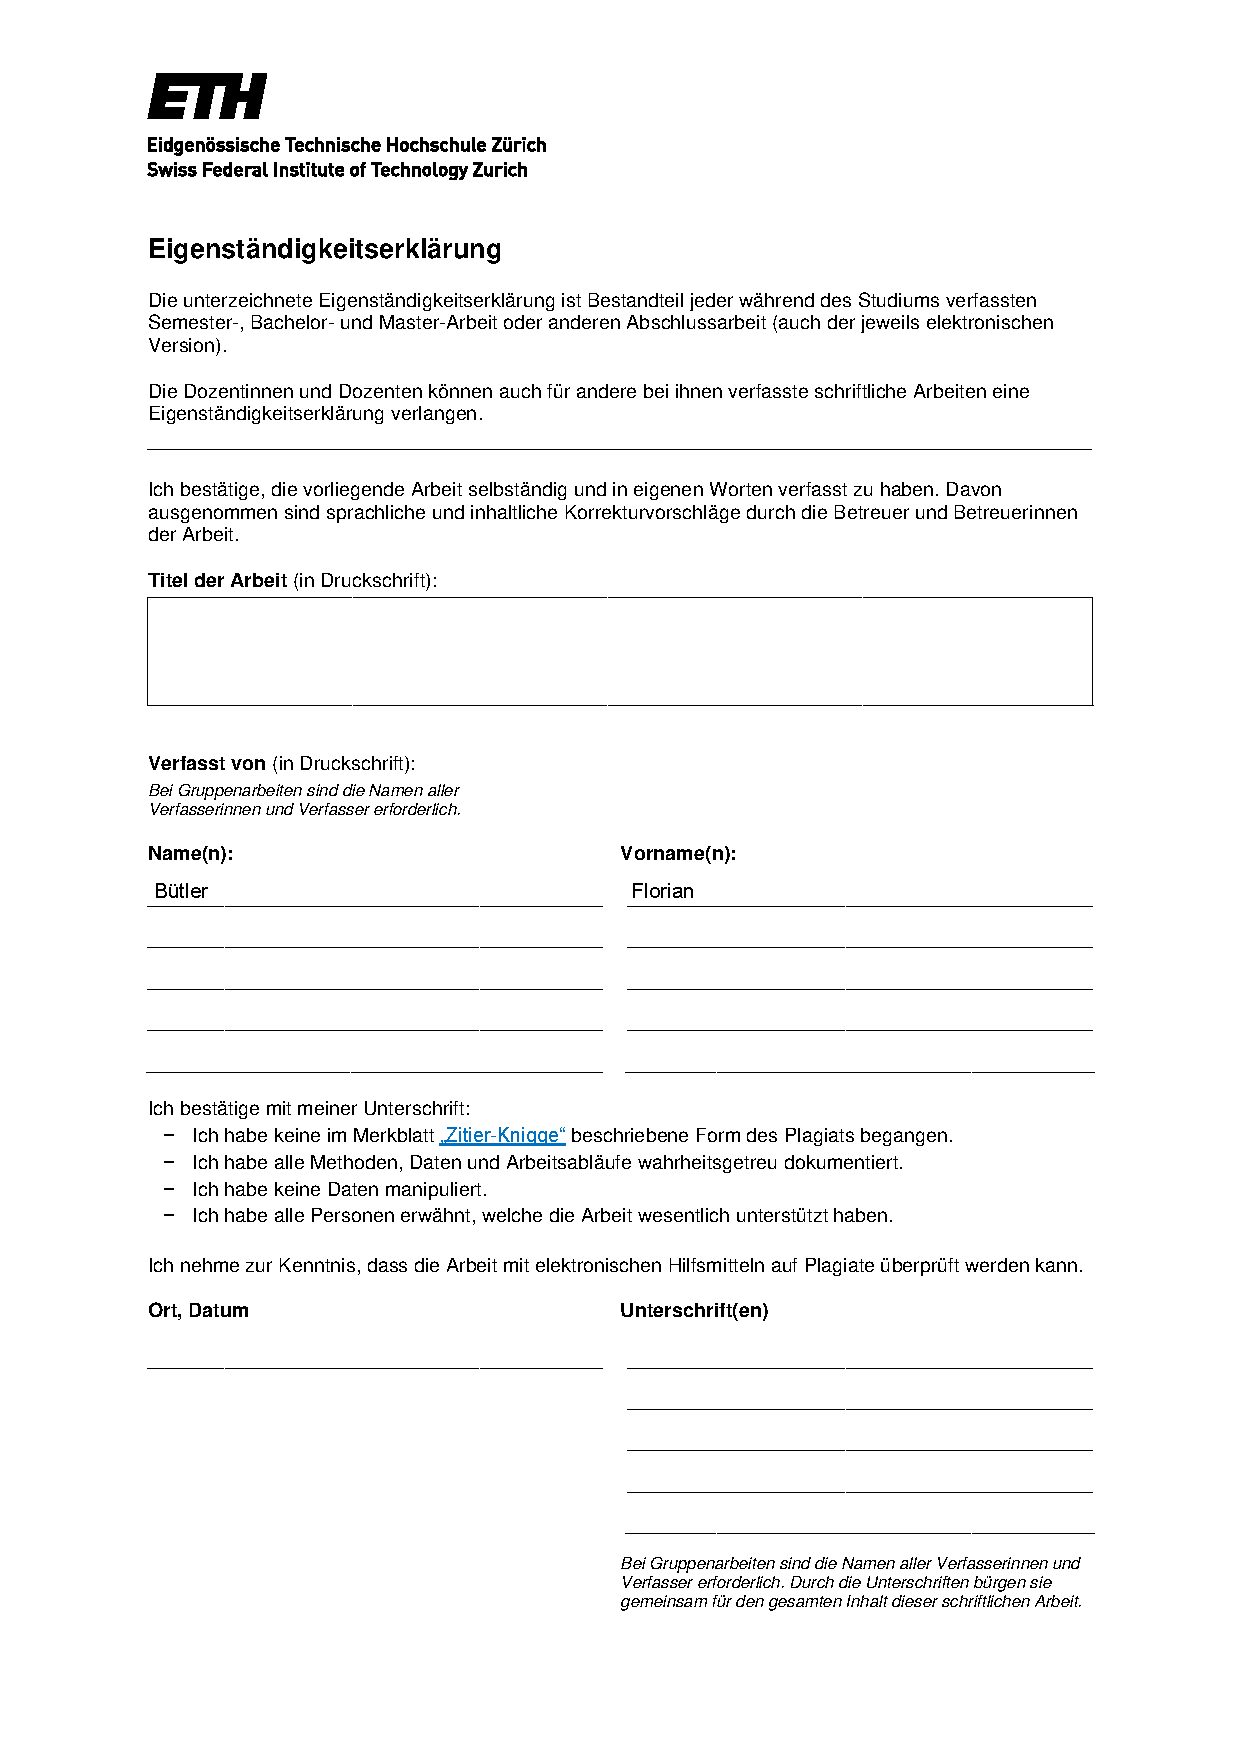
\includepdf[pages={1-},scale=1]{pdf/originality.pdf}

% This creates an appendix chapter, comment if not needed.
\appendix
\chapter{First Chapter Title}

Lorem ipsum dolor sit amet, consetetur sadipscing elitr, sed diam nonumy
eirmod tempor invidunt ut labore et dolore magna aliquyam erat, sed diam
voluptua.\TODO{This is a TODO annotation.}

\section{First Section Title}

Lorem ipsum dolor sit amet, consetetur sadipscing elitr, sed diam nonumy
eirmod tempor invidunt ut labore et dolore magna aliquyam erat, sed diam
voluptua.

\subsection{First Subsection Title}

Lorem ipsum dolor sit amet, consetetur sadipscing elitr, sed diam nonumy
eirmod tempor invidunt ut labore et dolore magna aliquyam erat, sed diam
voluptua.\REMARK{This is a REMARK annotation.}

\begin{theorem}[First Theorem] \label{thm:first theorem} This is our first
theorem. \end{theorem}

\begin{proof} And this is the proof of the first theorem with a complicated
formula and a reference to Theorem \ref{thm:first theorem}. Lorem ipsum dolor
sit amet, consetetur sadipscing elitr, sed diam nonumy eirmod tempor invidunt
ut labore et dolore magna aliquyam erat, sed diam voluptua. Lorem ipsum dolor
sit amet, consetetur sadipscing elitr, sed diam nonumy eirmod tempor invidunt
ut labore et dolore magna aliquyam erat, sed diam voluptua. \begin{equation}
{\frac {\mathrm d}{\mathrm dx}}\arctan(\sin({x}^{2}))=-2 \cdot {\frac
{\cos({x}^{2})x}{-2+\left (\cos({x}^{2})\right )^{2}}} \end{equation}
\end{proof}

\begin{lemma} lorem ipsum dolor sit amet \end{lemma}

\begin{corollary} lorem ipsum dolor sit amet \end{corollary}

\begin{observation} lorem ipsum dolor sit amet \end{observation}

\begin{definition} lorem ipsum dolor sit amet \end{definition}

\begin{problem} lorem ipsum dolor sit amet \end{problem}

\begin{assumption} lorem ipsum dolor sit amet \end{assumption}

\begin{example} lorem ipsum dolor sit amet \end{example}

\begin{claim} lorem ipsum dolor sit amet \end{claim}

\begin{remark} lorem ipsum dolor sit amet \end{remark}

Note that in \LaTeX, ``quotes'' do not use the usual double quote characters.

\end{document}